\documentclass[11pt,letterpaper]{article}
\usepackage[margin=1in]{geometry}
\usepackage{amsmath,amssymb,graphicx,booktabs}
\usepackage[T1]{fontenc}
\usepackage{lmodern,microtype}
\usepackage[hidelinks]{hyperref}
\hypersetup{pdftitle={Decision stumps as exact Maxwell fronts},pdfauthor={Jonathan R. Landers}}
\setlength{\parindent}{0pt}
\setlength{\parskip}{5pt}
\setlength{\abovedisplayskip}{6pt}
\setlength{\belowdisplayskip}{6pt}
\renewcommand{\topfraction}{0.9}
\renewcommand{\textfraction}{0.08}
\renewcommand{\floatpagefraction}{0.85}
\clubpenalty=10000
\widowpenalty=10000
\newcommand{\E}{\mathbf E}
\newcommand{\B}{\mathbf B}
\newcommand{\ind}{\mathbf1}
\newcommand{\TV}{\operatorname{TV}}
\begin{document}
\begin{center}
{\Large\bfseries Decision stumps as exact Maxwell fronts}\\[4pt]
{\normalsize Exact propagation does not guarantee the best learned waveform}\\[6pt]
Jonathan R. Landers
\end{center}

\textbf{Abstract.}
An exact physical representation need not be the best way to learn a field from data.
A correctly polarized decision stump moving at light speed is an exact weak
Maxwell solution. We derive a threshold representation of bounded-variation
waves and error bounds that persist under propagation. In two exploratory tests,
spatial trees trail Gaussian and dipole models on magnetic measurements, while
phase-based stumps fit a noisy pulse less accurately than a phase-based forest
(6.28\% versus 3.75\% error). Both phase models propagate exactly. The result
separates physical validity from predictive accuracy: equivalent representations
need not be equally compact or easy to learn.

\textbf{1. What does the staircase approximate?}
\emph{A finite staircase can obey Maxwell exactly and still fit the observed wave
less accurately than another model.} A decision stump changes value at a threshold;
adding stumps gives steps where a smooth wave oscillates continuously. Yet matching
that waveform and satisfying its field equations are separate requirements.
Our experiments find no predictive advantage for the tested stump learner, while
confirming a useful guarantee: its prescribed propagation carries profile error
without growth. A forest in the same traveling coordinate shares that guarantee.

Section~5 of \emph{Equivalent Descriptions of Light}~[1] represents a sinusoid
as an average of thresholds. We ask whether each finite approximation is already
an exact Maxwell field, and whether that helps it learn from data. Characteristic
and jump-condition methods~[2] establish the representation; measured room fields
and a simulated pulse test prediction. The front construction assumes homogeneous
vacuum with no charges, currents, or boundaries, and light speed
$c=(\mu_0\varepsilon_0)^{-1/2}$. The room test concerns a static magnetic map,
so it compares predictors rather than measuring propagating fronts.

\textbf{2. Maxwell's equations allow sharp fronts.}
Take one transverse polarization, $\E=\hat{\mathbf x}E(z,t)$ and
$\B=\hat{\mathbf y}B(z,t)$. The divergence equations hold automatically because
the fields have no longitudinal component or transverse dependence. The curl
equations reduce to
\begin{equation}
 E_t+c^2B_z=0,\qquad B_t+E_z=0.
 \label{eq:maxwell}
\end{equation}
Subscripts denote partial derivatives. Adding and subtracting $c$ times the
second equation gives the characteristic variables
\begin{equation}
 w_\pm=E\pm cB,\qquad (w_\pm)_t\pm c(w_\pm)_z=0.
 \label{eq:characteristics}
\end{equation}
Thus $w_+$ translates right and $w_-$ left. Setting $w_-=0$ leaves
\begin{equation}
 \boxed{E(z,t)=f(z-ct),\qquad B(z,t)=f(z-ct)/c.}
 \label{eq:profile}
\end{equation}
For differentiable $f$, substitution gives $-cf'+cf'=0$ and $-f'+f'=0$.
No sinusoidal assumption was needed: Maxwell fixes the translation speed and
field ratio, while the initial profile supplies $f$.

What if $f$ jumps? Write $H(\xi-a)=\ind_{\xi\ge a}$ and take
$f(\xi)=\alpha H(\xi-a)$, where $a$ is a threshold and $\alpha$ an electric-field
amplitude. In distributions, $H'=\delta$, the unit point mass. With $\xi=z-ct$,
\begin{equation}
 E_t+c^2B_z=-c\alpha\delta(\xi-a)+c\alpha\delta(\xi-a)=0,
 \qquad B_t+E_z=-\alpha\delta(\xi-a)+\alpha\delta(\xi-a)=0.
 \label{eq:weak}
\end{equation}
The cancellation includes the front itself. A weak solution means these equations
hold after integration against every smooth, compactly supported test function;
it does not require an ordinary derivative at the jump.

Equivalently, let $[E]$ and $[B]$ be right-minus-left jumps across $z=st+a$.
The delta coefficients in Eq.~\eqref{eq:maxwell} give
\begin{equation}
 s[E]=c^2[B],\qquad s[B]=[E].
 \label{eq:jump}
\end{equation}
A nonzero jump therefore travels at $s=\pm c$; for $s=c$, $[B]=[E]/c$.
This is a one-wave Riemann problem: two constant initial states separated by
one interface, whose jump excites only the right-moving characteristic.
Each correctly paired stump is already a solved propagation problem.

\textbf{3. From one front to any bounded-variation profile.}
For a precise global statement, let $f$ be right-continuous on $\mathbb R$ with
finite total variation $V=\TV(f)$. This is the total accumulated absolute change,
including jumps. Its distributional derivative is a finite signed measure
$\mu=df$, and $f_-=\lim_{\xi\to-\infty}f(\xi)$ exists. Then
\begin{equation}
 f(\xi)=f_-+\int_{\mathbb R}H(\xi-a)\,\mu(da).
 \label{eq:stieltjes}
\end{equation}
Indeed, the integral is $\mu(( -\infty,\xi])=f(\xi)-f_-$.
This fixes the integration limits and baseline; a jump of size $\alpha$ is
an atom $\alpha\delta_a$, hence exactly one stump.
On a finite interval the corresponding formula uses $f(\ell)$ and
$\int_{(\ell,r]}H(\xi-a)\,df(a)$ for $\ell\le\xi\le r$.

For an absolutely continuous profile, $\mu(da)=f'(a)\,da$.
If thresholds $A_j$ are sampled independently from a probability density $p$
that is positive wherever $f'\ne0$, define
\begin{equation}
 T_a(\xi)=\frac{f'(a)}{p(a)}H(\xi-a),\qquad
 \widehat f_N(\xi)=f_-+\frac1N\sum_{j=1}^N T_{A_j}(\xi).
 \label{eq:forest}
\end{equation}
Integration gives $\mathbb E\widehat f_N=f$. More fundamentally,
Eq.~\eqref{eq:weak} and linearity show that \emph{every realized finite sum},
with any fitted or chosen amplitudes, gives an exact weak Maxwell field through
Eq.~\eqref{eq:profile}. Randomness is a way to approximate the profile, not a
condition for physical validity. Here ``forest'' means this additive ensemble
of stumps; it need not be a conventionally trained random forest.

\textbf{4. How much waveform error survives?}
The measure form also supplies a clean uniform bound. Split
$\mu=\mu^+-\mu^-$ into its positive and negative parts, with masses
$V_+,V_-$ and $V_++V_-=V$. For each nonzero part draw $N$ independent
thresholds from $\mu^\pm/V_\pm$, and let $\widehat F_\pm$ be their empirical
cumulative distribution functions. Then
\begin{equation}
 \widehat f=f_-+V_+\widehat F_+-V_-\widehat F_-,\qquad
 \Pr\!\left\{\|\widehat f-f\|_\infty
 \le V\sqrt{\frac{\log(4/\delta)}{2N}}\right\}\ge1-\delta.
 \label{eq:dkw}
\end{equation}
To prove this, the Dvoretzky--Kiefer--Wolfowitz inequality with Massart's
constant~[3] bounds each CDF error above $\eta$ by $2e^{-2N\eta^2}$.
A union bound and the triangle inequality give Eq.~\eqref{eq:dkw}.
There are at most $2N$ stumps. For a monotone profile only one part is needed,
and $\log(4/\delta)$ becomes $\log(2/\delta)$. Atoms are allowed.

For the single-density estimator in Eq.~\eqref{eq:forest}, choosing
$p=|f'|/V$ makes the nonzero weights have magnitude $V$.
Cauchy--Schwarz gives $\int f'^2/p\,da\ge(\int|f'|\,da)^2=V^2$.
Thus this choice minimizes a common second-moment bound for all thresholds
$\xi$; it need not minimize variance at a particular query, where only $a\le\xi$
contribute. The two-CDF construction avoids that ambiguity for general BV data.

The dynamical conclusion is deterministic. Translation preserves the supremum
norm, so on the whole line, at every time,
\begin{equation}
 \|\widehat E(\cdot,t)-E(\cdot,t)\|_\infty
 =\|c\widehat B(\cdot,t)-cB(\cdot,t)\|_\infty
 =\|\widehat f-f\|_\infty.
 \label{eq:transporterror}
\end{equation}
The probability bound therefore holds simultaneously for all times, with no
new sampling. A detector sees waveform error, but that error does not grow
through propagation.

\textbf{5. A sinusoid, a wrap point, and energy.}
An eternal sinusoid is not globally BV. Work instead on one period and use the
dimensionless phase $q=(kz-ckt)\bmod 2\pi$, with $k>0$. For uniform
$A\in[0,2\pi)$,
\begin{equation}
 \mathbb E[2\pi\cos A\,\ind_{q\ge A}]
 =\int_0^q\cos a\,da=\sin q.
 \label{eq:sine}
\end{equation}
Multiplying this profile by an amplitude $E_0$ gives
$E=E_0\sin q$ and $B=E/c$. Each periodically repeated stump has both its
threshold jump and a reset at the wrap. Both move at $c$, so a finite sample
remains an exact weak solution, even when its reset jumps do not cancel.
The target's continuous wrap follows from $\int_0^{2\pi}\cos a\,da=0$.

Cancellation can also be enforced at finite size: the positive and negative
derivative masses of $\sin q$ are both $2$. Sampling $N$ thresholds from each
normalized part gives $\widehat f=2\widehat F_+-2\widehat F_-$, with zero
net jump over a period. Equation~\eqref{eq:dkw} applies on that period with
$V=4$, and periodicity extends it to all phase values and times.
This gives a continuous match across the wrap without removing the interior steps.

For a right-moving field, the electromagnetic energy density and flux are
$u=\varepsilon_0E^2$ and $S_z=cu$. If $|E|\le M$ and
$|\widehat E-E|\le\epsilon$, then
\begin{equation}
 |\widehat u-u|\le\varepsilon_0\epsilon(2M+\epsilon),\qquad
 |\widehat S_z-S_z|\le c\varepsilon_0\epsilon(2M+\epsilon).
\end{equation}
These are local bounds. A single step has infinite longitudinal energy, and
all plane waves extend infinitely across the transverse plane. Finite pulse
energy per unit transverse area is possible: the paired fronts
$f=E_0[H(\xi-a)-H(\xi-b)]$, $a<b$, form a rectangular pulse with
$\int u\,dz=\varepsilon_0E_0^2(b-a)$. Claims about total energy require such
tail cancellation or appropriate integrability, beyond a uniform error bound.

\textbf{6. Which geometry and which physics are built in?}
For a unit direction $\mathbf n$ and constant polarization $\mathbf e$ with
$\mathbf n\cdot\mathbf e=0$, a three-dimensional front is
\begin{equation}
 \E=\mathbf e H(\phi),\qquad
 \B=\frac{\mathbf n\times\mathbf e}{c}H(\phi),\qquad
 \phi=\mathbf n\cdot\mathbf x-ct-a.
 \label{eq:null}
\end{equation}
The divergence coefficients vanish by transversality. The curl equations follow
from $\mathbf n\times(\mathbf n\times\mathbf e)=-\mathbf e$, giving
$\E_t=c^2\nabla\times\B=-c\mathbf e\delta(\phi)$ and
$\B_t=-\nabla\times\E=-(\mathbf n\times\mathbf e)\delta(\phi)$.
In coordinates $(\mathbf x,ct)$ the front normal $(\mathbf n,-1)$ has
Minkowski squared norm $|\mathbf n|^2-1=0$: the split is lightlike.

Any finite additive superposition of these polarized fronts is exact, including
different directions. A deeper tree needs more care: null split surfaces alone
do not guarantee compatible field jumps between its leaves. Every interface
must satisfy the Maxwell jump conditions. Nor does this establish that finite
plane-front sums are dense in the global finite-energy solution space; the
individual fronts generally lie outside that space. The one-dimensional
extension is direct. Given initial fields $E_i(z),B_i(z)$,
define $g_\pm(z)=E_i(z)\pm cB_i(z)$. Equation~\eqref{eq:characteristics} yields
\begin{equation}
 E(z,t)=\frac{g_+(z-ct)+g_-(z+ct)}2,\qquad
 cB(z,t)=\frac{g_+(z-ct)-g_-(z+ct)}2.
\end{equation}
Two forests therefore represent both directions whenever $g_\pm$ have the stated
BV regularity. The other transverse polarization works the same way; constant
longitudinal backgrounds can be added.

Exactness also depends on the propagation law. The ideal LC chain in~[1], with
spacing $d$, inductance $L$, and capacitance $C$, has dispersion
$\Omega^2=4\sin^2(kd/2)/(LC)$. Only at long wavelengths does this become
$\Omega^2\simeq v^2k^2$, where $v=d/\sqrt{LC}$. A sharp translating step
contains short wavelengths and cannot retain its continuum shape on that
lattice. A step therefore probes the limits of the continuum description.

\textbf{7. What does the representation teach us?}
The earlier companion studies follow samples into fitted functions, selected
equations, and equivalent magnetic sources~[4--6]. The dipole model supplies
magnetostatic responses and learns their coefficients; its measurement-weight
form makes that dependence exact~[6]. Stump fronts supply a time-dependent
counterpart: fitting amplitudes or thresholds changes the predicted wave while
preserving the supplied vacuum equations. Neither construction discovers those
equations merely by using their solutions. Sparse measurements can still leave
many admissible fields, and the sampling bound above concerns a known profile,
not recovery from noisy sensors.

An illustrative learning problem can nevertheless be stated concretely. Fix thresholds $a_j$
and observe noisy electric readings $y_i$ at positions and times $(z_i,t_i)$.
For a right-moving model, set $X_{i0}=1$ and
$X_{ij}=H(z_i-ct_i-a_j)$ for $j\ge1$. One possible fit is
\begin{equation}
 \widehat{\boldsymbol\beta}
 =\underset{\boldsymbol\beta}{\arg\min}\left\{
 \|X\boldsymbol\beta-\mathbf y\|_2^2
 +\lambda\sum_{j=1}^{m}\beta_j^2\right\},\qquad
 \widehat f(\xi)=\widehat\beta_0+
 \sum_{j=1}^{m}\widehat\beta_jH(\xi-a_j),\quad\lambda>0.
\end{equation}
The constant background is unpenalized. Setting $\widehat E=\widehat f(z-ct)$
and $\widehat B=\widehat E/c$ preserves Maxwell for every fitted coefficient
vector. Validation must still choose useful thresholds and regularization,
and test whether a single propagation direction describes the readings.
Unlike the profile-sampling construction, this fit does not know $df$ in advance.
Its errors involve sensor noise and coverage as well as finite representation.
Several observations at different places and times may share the same phase
$z_i-ct_i$; they then constrain the same profile value rather than supplying
new spatial detail. The physical basis guarantees an admissible evolution,
while the experiment determines how much of that evolution is identifiable.
The experiments below use tree boosting and random forests rather than this
fixed-threshold ridge estimator. None samples from a known derivative measure,
so the DKW bound in Section~4 is not a statistical guarantee for these fitted models.

\textbf{8. Experiment I: predicting the measured magnetic map.}
The Aalto recordings~[7] pair planar positions with three magnetic channels.
We reuse the earlier papers' exact arrays and calibration~[5,6]: 500 training
readings from trials~1--2, 600 validation readings from trial~3, stable tests
on trials~4--5, and changed-environment tests on trials~6--9. Each instrument
contributes 3,000 stable and 6,000 changed-test readings. A predefined rectangle
and 0.15~m buffer are excluded from training and validation to test spatial
transfer. Other instruments retain their trial-1-only calibration.

Both tree models take $(x,y)$ as input. A 150-tree forest predicts the three
channels jointly; boosted depth-one trees fit them separately. Validation
searches 18 forest settings and nine boosting settings, selecting by mean
error across seeds 11, 23, and 37. The selected forest has unrestricted depth,
leaf size one, and feature fraction 0.7; the stumps use 200 stages at rate 0.03.
Full parameter grids are retained with the results. Earlier Gaussian and dipole
predictions are reused unchanged and checked against their published scores.
For readings $\mathbf b_i$, vector RMSE is
\begin{equation}
 R=\left(\frac1n\sum_{i=1}^n
 \|\widehat{\mathbf b}_i-\mathbf b_i\|_2^2\right)^{1/2}.
 \label{eq:sensor-rmse}
\end{equation}
Errors retain reference recording units. Across all instruments and both
environments, trees improve on the constant predictor but trail the Gaussian
and dipole models (Table~\ref{tab:sensors}). Stable reference-instrument RMSE is
14.70 for stumps, 10.56 for the forest, 8.09 for the Gaussian, and 5.22 for
kernel-to-dipoles. Forest seed standard deviations are 0.03 for stable data
and 0.06 for changed data; stump predictions are identical across seeds.
These spreads measure algorithm variation, not uncertainty across rooms.

\begin{table}[tbp]
\centering\small
\begin{tabular}{llrrrrr}
\toprule
Environment & Instrument & Stumps & Forest & Gaussian & Direct & Two-stage\\
\midrule
Stable & Invensense & 14.70 & 10.56 & 8.09 & 5.31 & 5.22\\
Stable & Nexus & 14.72 & 11.77 & 10.34 & 8.85 & 8.83\\
Stable & Trivisio & 14.62 & 10.20 & 8.03 & 5.71 & 5.56\\
Changed & Invensense & 16.15 & 10.82 & 8.64 & 7.36 & 7.33\\
Changed & Nexus & 27.01 & 25.29 & 24.16 & 23.79 & 23.81\\
Changed & Trivisio & 16.01 & 10.58 & 8.69 & 7.50 & 7.43\\
\bottomrule
\end{tabular}

\caption{Magnetic-map vector RMSE; lower is better. Tree entries average three
seeds. ``Direct'' fits dipoles to readings; ``Two-stage'' fits them to Gaussian
predictions. Test arrays and alignment match the earlier studies.}
\label{tab:sensors}
\end{table}

\begin{figure}[tbp]
\centering
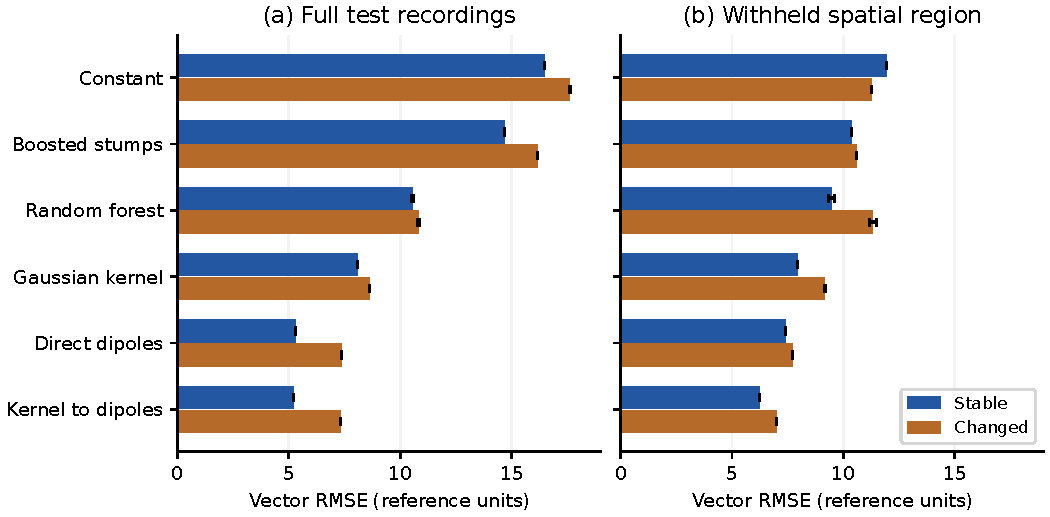
\includegraphics[width=\linewidth]{stump_sensor_comparison.pdf}
\caption{Reference-instrument RMSE on (a) full recordings and (b) the withheld
rectangle, containing 354 stable and 545 changed-environment readings. Error
bars show tree-seed standard deviations; earlier baselines are single fits.
These static-map tests do not measure propagating Maxwell fronts.}
\label{fig:sensors}
\end{figure}

The withheld region gives the same ordering (Figure~\ref{fig:sensors}): stable
reference errors are 10.38 for stumps, 9.46 for the forest, 7.95 for the Gaussian,
and 6.24 for kernel-to-dipoles. Thus the earlier dipole advantage persists against
additional statistical baselines. This does not test the front theorem: spatial
trees lack its traveling phase and field coupling. Axis-aligned stump sums also
restrict each component to $b_0+g(x)+h(y)$, whereas deeper trees allow spatial
interactions. Oblique stumps and broader fitting searches remain untested.

\textbf{9. Experiment II: fitting a traveling pulse.}
The second test addresses the front construction directly. In dimensionless
units set $c=1$, write $C=cB$ so the two channels have common units, and choose
\begin{equation}
 f(\xi)=e^{-(\xi/0.7)^2}\cos(4\xi),\qquad
 \xi=z-t,\qquad E(z,t)=C(z,t)=f(\xi).
 \label{eq:test-pulse}
\end{equation}
For each seed, draw 600 training and 300 validation points uniformly from
$z\in[-3,4]$, $t\in[0,1]$, retaining $\xi\in[-3,3]$. Add independent Gaussian
noise to both channels at 2\% of clean training component RMS. Generic forests
and boosted stumps take $(z,t)$ and predict $(E,C)$. Two constrained models
instead take the supplied phase $\xi$, fit the averaged target $(y_E+y_C)/2$,
and set $\widehat E=\widehat C$: boosted stumps and a random forest.
Both receive the same speed, direction, field coupling, and noise averaging.

The recorded parameter grids are selected independently per seed using noisy
validation data. Phase stumps select 600 stages at rate 0.3; phase forests select
depth 12 and leaf size one. The phase-forest control was added after inspecting
the initial results, so this is exploratory, although future labels never select
settings. Score noiseless fields at $t=0,0.5,1,2,4$ on the same 2,401-point
phase grid, placing queries at $z=\xi+t$. Later queries also partly leave the
generic models' training spatial range. For $\mathbf U=(E,C)$, relative error is
\begin{equation}
 r(t)=\frac{\left(\sum_i\|\widehat{\mathbf U}(\xi_i+t,t)
             -\mathbf U(\xi_i+t,t)\|_2^2\right)^{1/2}}
 {\left(\sum_i\|\mathbf U(\xi_i+t,t)\|_2^2\right)^{1/2}}.
 \label{eq:relative-error}
\end{equation}
This approximates an $L^2$ ratio on the phase window. Table~\ref{tab:wave}
reports means and sample standard deviations, not confidence intervals.

\begin{table}[tbp]
\centering\small
\begin{tabular}{lrrr}
\toprule
Model & $t=0.5$ & $t=2$ & $t=4$\\
\midrule
Forest on (z,t) & $29.55\pm5.39$ & $130.91\pm4.05$ & $107.75\pm1.38$\\
Stumps on (z,t) & $64.92\pm0.39$ & $164.36\pm89.50$ & $163.14\pm99.00$\\
Stumps on phase & $6.28\pm1.34$ & $6.28\pm1.34$ & $6.28\pm1.34$\\
Forest on phase & $3.75\pm2.15$ & $3.75\pm2.15$ & $3.75\pm2.15$\\
\bottomrule
\end{tabular}

\caption{Relative field error (\%), mean $\pm$ sample standard deviation across
three seeds. Training uses $0\le t\le1$; every test uses the same phase window.
Both phase models share the supplied propagation law and field coupling.}
\label{tab:wave}
\end{table}

\begin{figure}[tbp]
\centering
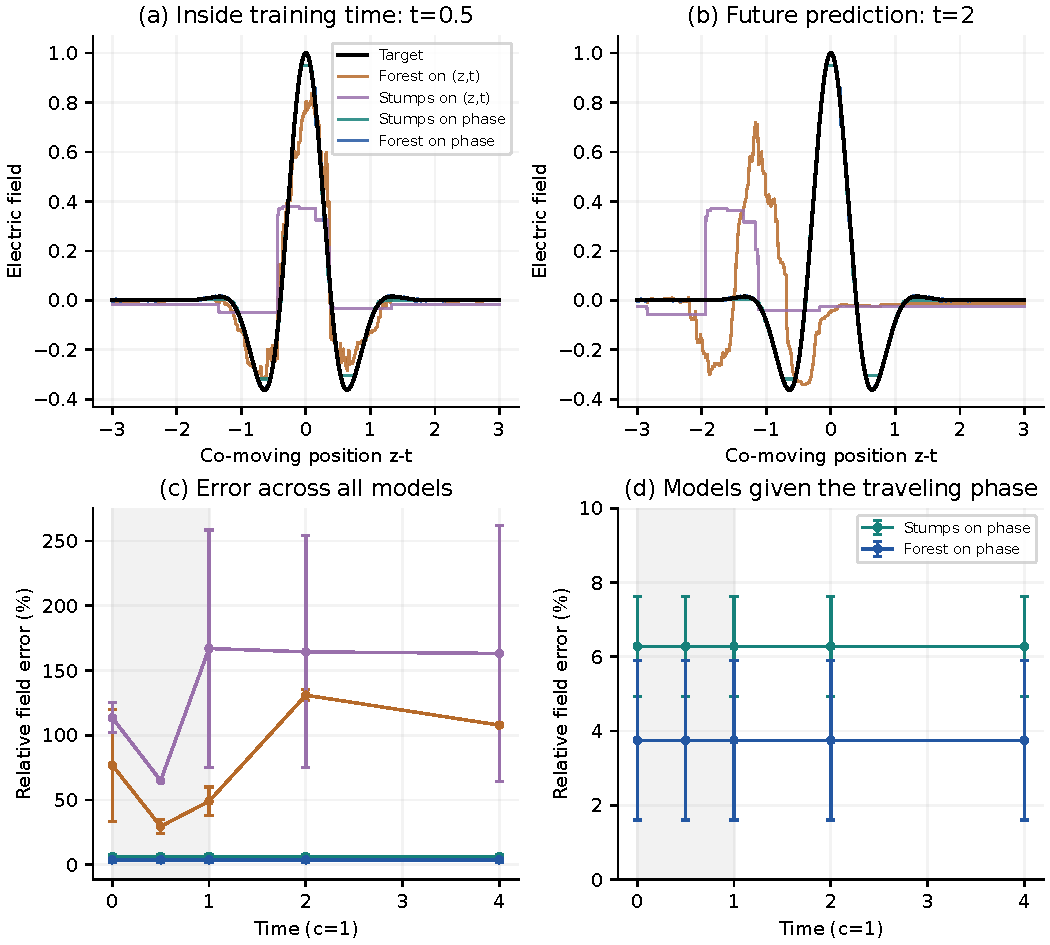
\includegraphics[width=\linewidth]{stump_wave_comparison.pdf}
\caption{(a,b) Electric-field predictions for fixed seed 11, inside the training
time interval and later. (c) Mean relative field errors with sample standard
deviations; shading marks training times. (d) An expanded scale separates the
phase models. Their errors stay constant because their fitted profiles translate.}
\label{fig:wave}
\end{figure}

Phase stumps attain $6.28\pm1.34$\% error at every time; the phase forest attains
$3.75\pm2.15$\% and wins on each seed. The generic forest rises from 29.55\%
at $t=0.5$ to 130.91\% at $t=2$, while generic stumps perform worse
(Figure~\ref{fig:wave}). The generic fits do not reliably propagate the pulse.

\emph{Checking the equations separately.}
Extracting each constrained stump's threshold and jump reproduces saved
predictions to tolerance $10^{-12}$. For $c=1$, the distributional residual
coefficients at a front moving at speed $s$ are
\begin{equation}
 \mathbf r_{\rm jump}=(-s[E]+[C],\,-s[C]+[E]).
\end{equation}
All 600 stages per seed have $[E]=[C]=\alpha_j$ and $s=1$, giving zero residual.
Changing $s$ to 0.8 gives $0.2\alpha_j(1,1)$, with maximum absolute coefficients
0.00797--0.01129 across seeds. This checks the analytical cancellation, not
Maxwell's law independently. Both phase models also preserve identical
co-moving predictions and $\widehat E=\widehat C$ at all five times.

\textbf{10. The negative result and what survives it.}
The tested stump learner wins neither experiment. That is a negative result
for these fitting procedures, not proof that stumps are intrinsically inferior.
The comparisons use one room dataset, one pulse family, and finite parameter
searches; sensor tests were previously examined and the phase control was added
during the investigation.

Moreover, a one-dimensional forest is itself a stump representation. It is
constant between the union of its trees' thresholds $a_1<\cdots<a_K$.
With successive levels $v_0,\ldots,v_K$, its profile is
\begin{equation}
 g(\xi)=v_0+\sum_{j=1}^K(v_j-v_{j-1})H(\xi-a_j).
 \label{eq:forest-as-stumps}
\end{equation}
Threshold values do not affect the weak field. The better phase forest therefore
also gives an exact weak Maxwell solution, using potentially different complexity
and regularization from the booster. The two methods are not disjoint
representation classes.

The interesting distinction is between \emph{admissibility}, \emph{estimation},
and \emph{economy}. The equations guarantee a permitted evolution; data determine
which profile to choose; the representation determines how compactly it is
expressed. One sine function describes a sinusoid that generally needs an infinite
stump superposition. Equivalence does not guarantee equal simplicity or learning
efficiency. Yet even an imperfect fitted staircase can propagate without further
profile error, which is the construction's precise benefit.

That guarantee assumes the correct phase and field coupling. It does not imply
discovery of Maxwell, a DKW bound for boosted fits, or validity in dispersive
media. The finite-window pulse scores also imply no total-energy convergence,
since fitted trees may retain constant tails. Smooth phase estimators and matched
complexity comparisons remain useful controls. The dipole advantage on the room
recordings likewise supports that static-field model within its tested scope,
not a universal ranking of physical and statistical descriptions.

\textbf{11. Takeaways.}
A moving decision stump can be an exact weak Maxwell front. A finite ensemble
can approximate a smooth waveform while satisfying the equations exactly.
The negative finding concerns the tested learner: the better phase forest
belongs to the same stump-representable class. Equivalence preserves dynamics,
not simplicity or statistical efficiency. Assess a representation twice:
what physics does it guarantee, and how well do data determine its field?

\textbf{Reproducibility.}
\begingroup\raggedright
Predictions, validation candidates, scores, and provenance are in
\path{experiments/magnetic_mapping/tree_comparison/}.
Run \path{experiments/magnetic_mapping/run_tree_comparison.py} to repeat fitting,
using \path{tree_requirements.txt} and the documented cached data.
The paper's \path{build_stump_assets.py} verifies hashes and generates figures
and tables without refitting. All 27 magnetic-mapping checks pass, including
score reconstruction, stump expansion, propagation invariance, and dipole
identities. Build instructions accompany the source.
\par\endgroup

{\footnotesize\raggedright
\textbf{References.}\par
[1] J. R. Landers, \href{equivalent_descriptions.pdf}{\emph{Equivalent Descriptions of Light}} (2026).\par
[2] D. I. Ketcheson, R. J. LeVeque, and M. J. del Razo,
\emph{Riemann Problems and Jupyter Solutions} (SIAM, 2020),
\href{https://www.clawpack.org/riemann_book/html/Acoustics.html}{linear systems and characteristics}.\par
[3] P. Massart, \emph{The tight constant in the Dvoretzky--Kiefer--Wolfowitz inequality},
Ann. Probab.\ \textbf{18}, 1269--1283 (1990),
\href{https://doi.org/10.1214/aop/1176990746}{doi:10.1214/aop/1176990746}.\par
[4] J. R. Landers, \href{../01-kernel-to-equation/kernel_to_equation.pdf}{\emph{From samples to an equation}};
\href{../03-maxwells-perspective/maxwells_perspective.pdf}{\emph{Maxwell's Perspective}} (2026).\par
[5] J. R. Landers, \href{../02-kernel-to-magnetostatics/kernel_to_magnetostatics.pdf}{\emph{From a learned kernel to a magnetic field}} (2026).\par
[6] J. R. Landers, \href{../04-measurement-influence/measurement_influence.pdf}{\emph{The magnetic field as a learned function}};
\href{../arxiv-draft-maxwell/arxiv-draft.pdf}{\emph{Magnetic Fields from Measurements}} (2026).
\par
[7] A. Solin, M. Kok, N. Wahlstr\"om, T. B. Sch\"on, and S. S\"arkk\"a,
\emph{Modeling and interpolation of the ambient magnetic field by Gaussian processes},
IEEE Trans.\ Robotics \textbf{34}, 1112--1127 (2018),
\href{https://doi.org/10.1109/TRO.2018.2830326}{doi:10.1109/TRO.2018.2830326};
\href{https://github.com/AaltoML/magnetic-data}{authors' public recordings}.
}
\end{document}
